\documentclass[twoside,10pt]{article}
\usepackage{amsmath,amsfonts,amsthm,fullpage}
\usepackage{algorithm}
\usepackage{algorithmic}
\usepackage{graphicx}
\usepackage{hyperref}
\usepackage{enumitem}

\setlist[itemize]{noitemsep, topsep=0pt}
\raggedbottom


\begin{document}

\title{ISYE 6740 Fall 2025\\ Homework 1 (100 points)\\Student Name Here}
%\author{Yao Xie}
\date{}

\maketitle

\vspace{-.5in}

In this homework, the superscript of a symbol $\text x^i$ denotes the index of samples (not raising to $i$th power); this is a convention in this class. Please follow the homework submission instructions in the syllabus.
\newline
\newline
\textbf{Provided Data:}
Questions marked with GS must be submitted to Gradescope. You must still include all your results and explanations in this PDF, and include your code in your submitted zip. Failure to pass all gradescope tests will result in losing 50\% of the points for that question.
\begin{itemize}
    \item (GS) Q3: Image compression using clustering [football.bmp, parrots.png]
    \item (GS) Q4: Political Blogs Spectral Clustering [nodes.txt, edges.txt]
    \item Q5: AI model compression [AImodel.npy]
\end{itemize}

\leavevmode\newline
\textbf{All results that are present only in code/notebooks, but not in your PDF report will not be accepted for points. Handwritten answers will not receive credit.}


\section{Concept questions [25 points]}

Please provide a brief answer to each question, and provide math arguments if asked. 

\begin{enumerate}


\item (5 points) Consider a dataset with data points each having 3 features, e.g., $x^1 = \{\mbox{``Atlanta''}, \mbox{``house''}, 500k\}$, and $x^2 = \{\mbox{``Dallas''}, \mbox{``house''}, 300k\}$. Define a proper similarity function $d(x^i, x^j)$ for this kind of data, and argue why it is a reasonable choice. (Hint: The feature vector consists of categorial and real-valued features; for categorical variables, it is better to convert them into one-hot-keying binary vectors and use Hamming distance, and for real-valued features, you may use Euclidean distance, for instance. And then you can combine the similarity measure in some way.)

\item (5 points) Show that the clustering assignment problem 
\[
\pi(i) = \arg\min_{j=1, \ldots, k} \|x^i- c^j\|^2
\]
is equivalent to solving
\[
\pi(i) = \arg \min_{j=1, \ldots, k} (c^j)^T\left(\frac 1 2 c^j-x^i\right).
\]
Note that the second approach will facilitate ``vectorized'' operation and be implemented in our demo code. 



\item (5 points) Why do different initializations for k-means lead to different results? In practice, to finding a better result facing this issue, what would you do?

\item (5 points) Why $k$-means will not have the issue of running a infinite number of iterations (suppose the stopping criterion is when the cluster assignments after another iteration do not change), in most settings?

\item (5 points) Consider the following simple graph
\begin{center}
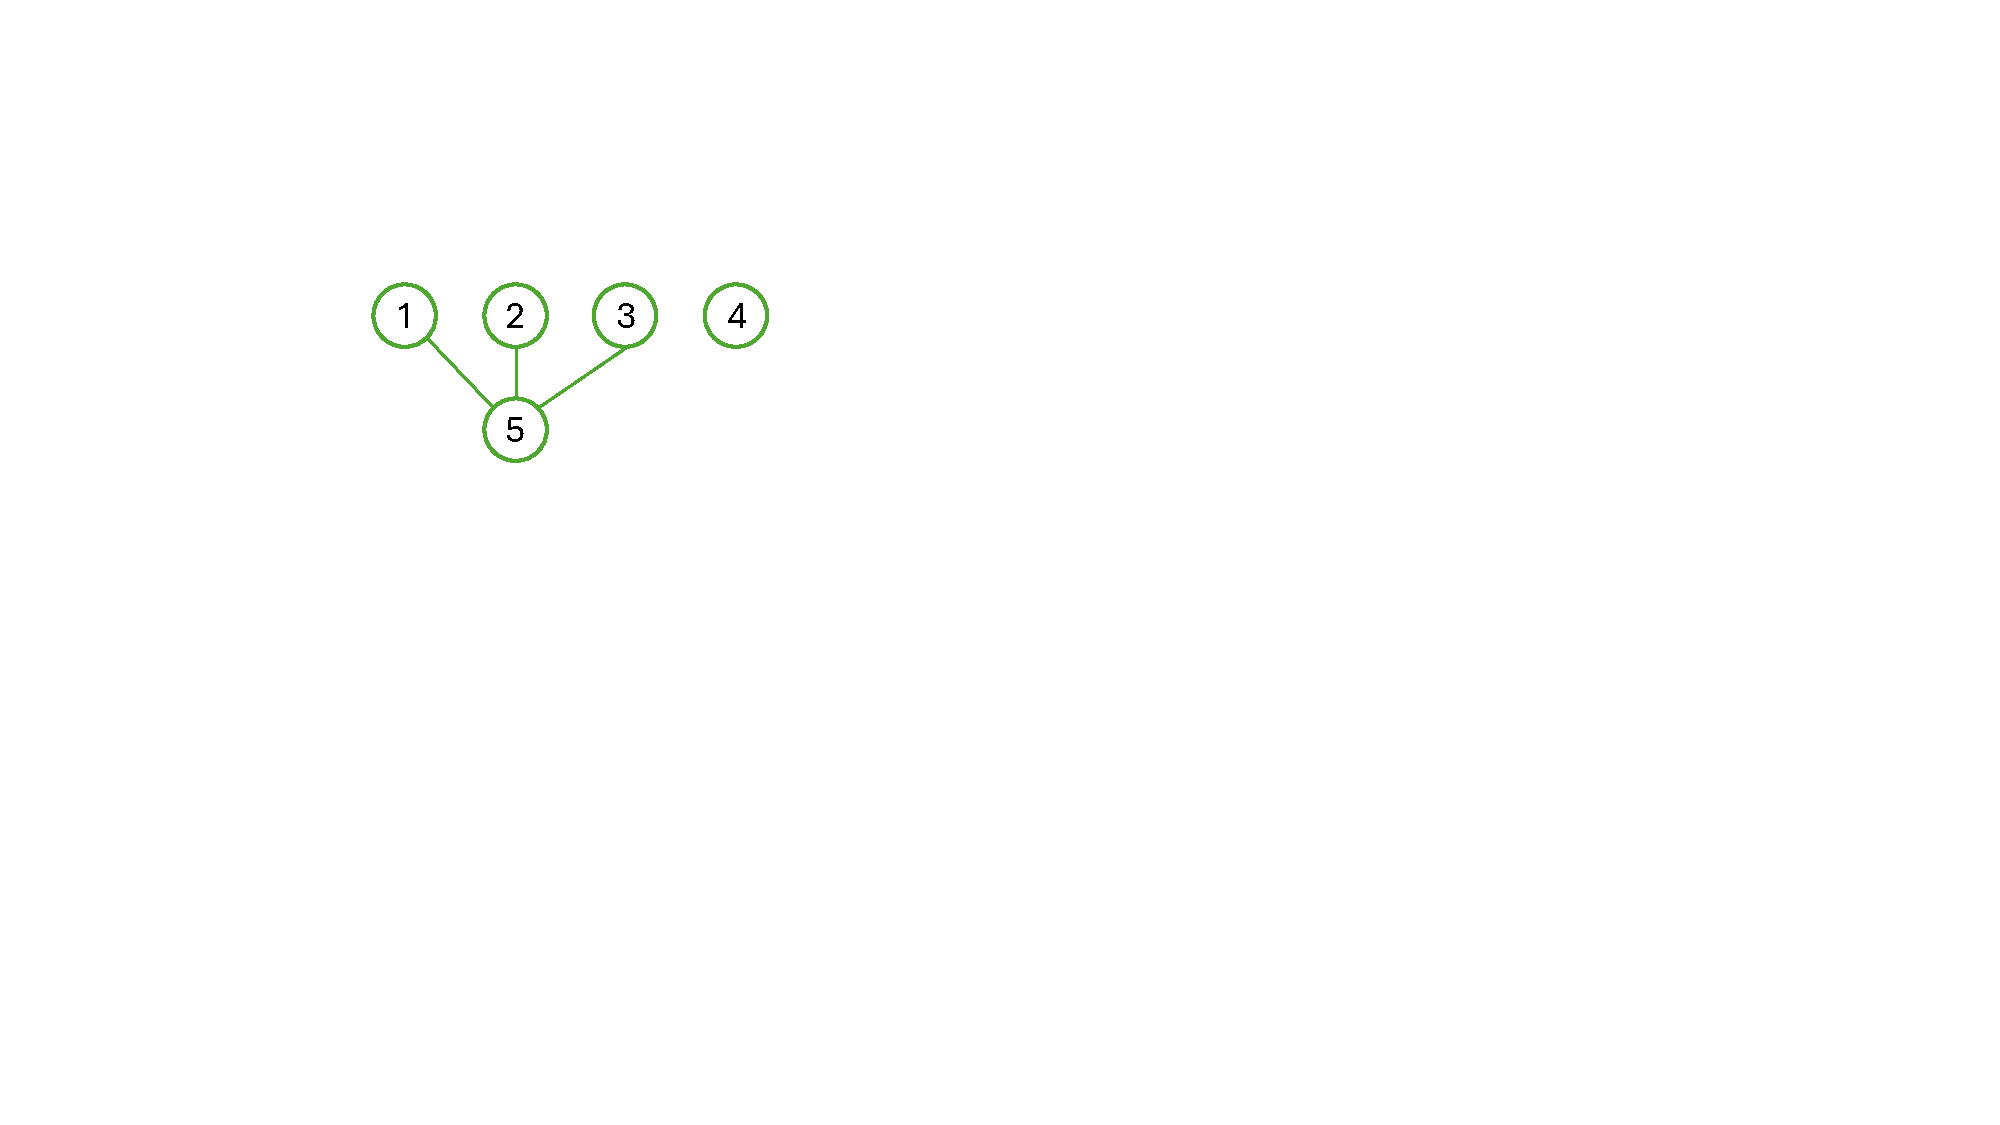
\includegraphics[width = 0.4\textwidth]{diag_ver2.pdf}
\end{center}

Write down the graph Laplacian matrix and find the eigenvectors associated with the zero eigenvalues. Explain how you find out the number of disconnected clusters in the graph and identify these disconnected clusters using these eigenvectors.

\end{enumerate}

\section{Math of k-means clustering [20 points]}
 Given $m$ data points $\text x^i \in \mathbb R^{n}$, $i=1,\dots, m$, $K$-means clustering algorithm groups them into $k$ clusters by minimizing the distortion function over $\{ r^{ij}, \mu^j \}$
\begin{equation}
J = \frac{1}{mk}\sum_{i=1}^m\sum_{j=1}^k r^{ij} \|\text x^i-\mu^j\|^2,
\label{J_def}
\end{equation}
where $r^{ij}=1$ if $\text x^i$ belongs to the $j$-th cluster and $r^{ij}=0$ otherwise.

\begin{enumerate}

\item (8 points) Derive mathematically that using the squared Euclidean distance $\|\text x^i-\mu^j\|^2$ as the dissimilarity function, the centroid that minimizes the distortion function $J$  for given assignments $r^{ij}$ are given by
   $$\mu^j=\frac{\sum_i r^{ij} \text x^i}{\sum_i r^{ij}}.$$
   That is, $\mu^j$ is the center of $j$-th cluster.  \\
   Hint: You may start by taking the partial derivative of $J$ with respect to $\mu^j$, with $r^{ij}$ fixed.
   
   
\item (7 points) Derive mathematically what should be the assignment variables $r^{ij}$ be to minimize the distortion function $J$, when the centroids $\mu^j$ are fixed.

\item (5 points) For the question above, now suppose we change the similar score to a ``quadratic'' distance (also known as Mahalanobis distance) for given and fixed positive definite matrix $\Sigma \in \mathbb R^{n\times n}$, and the distortion function becomes:
\[
J = \frac{1}{mk}\sum_{i=1}^m\sum_{j=1}^k r^{ij} (\text x^i-\mu^j)^T \Sigma  (\text x^i-\mu^j),
\]
Derive what $\mu^{j}$ and $r^{ij}$ becomes in this case.

\end{enumerate}



\section{Image compression using clustering [20 points]}

In this programming assignment, you are going to apply clustering algorithms for image compression. This can also be viewed as an example of segmenting colors in an automated fashion using $K$-means clustering.

Your task is to implement \emph{$K$-means} for this purpose.  {\bf It is required you implement the algorithms yourself rather than calling k-means from a package. However, it is ok to use standard packages for supplementary tasks, e.g., file i/o, linear algebra, distance calculations, and visualization.} 


\subsubsection*{Formatting instruction}

As a starting point, we suggest the following input/output signature for your k-means algorithm.\\

\textbf{Input}
\begin{itemize}
  \item \texttt{pixels}: the input image representation. Each row contains one data point (pixel). For image dataset, it contains 3 columns, each column corresponding to Red, Green, and Blue components. Each component has an integer value between 0 and 255.
  \item \texttt{k}: the number of desired clusters.
\end{itemize}

\textbf{Output}
\begin{itemize}
  \item \texttt{class}: cluster assignment of each data point in pixels. The assignment should be 1, 2, 3, etc. For $k = 5$, for example, each cell of the class should be either 1, 2, 3, 4, or 5. The output should be a column vector with \texttt{size(pixels, 1)} elements.
  \item \texttt{centroid}: location of $k$ centroids (or representatives) in your result. With images, each centroid corresponds to the representative color of each cluster. The output should be a matrix with $K$ rows and 3 columns. The range of values should be [0, 255], possibly floating point numbers.
\end{itemize}

\subsubsection*{Hand-in}
Both your code and report will be evaluated. You must pass the gradescope unit tests to receive full credit, additionally upload your code into canvas and include your results in your PDF report separate from your code zip file. In your report, answer the following questions:

\begin{enumerate}
 
\item  (5 points) Use $k$-means with squared-$\ell_2$ norm as a metric for \texttt{parrots.png} and \texttt{football.bmp} and also choose a third picture of your own to work on. Your chosen image should meet the following requirements: 
\begin{itemize}
    \item Full Color (No black and white images)
    \item Recommended size between 200x150 and 400x300. Larger images are acceptable assuming they meet runtime requirements listed below in the Note, Smaller images are not acceptable.
\end{itemize}
Run your $k$-means implementation with these pictures, with several different $k = 3, 6, 12, 24, 48$.
  
{\it Comment:}  Your algorithm will segment the image into k regions in the RGB color space. For each pixel in the input image, the algorithm returns a label corresponding to a cluster.
  
Run your $k$-means implementation (with squared-$\ell_2$ norm) with random initialization centroids. Due to the nature of randomness, Please try multiple times and report the only the best seed (in terms of image quality). Please provide the following deliverables:
\begin{itemize}
    \item For every K on all 3 images, the reconstructed image
    \item The time in seconds it takes to converge for every K on each image
    \item The number of iterations to convergence for every K on each image
\end{itemize}
  
\item (10 points) Now adjust your k-means implementation to use the Manhattan distance ($\ell_1$ norm) metric. Please provide all of the same above deliverables for all three images. Provide a comment on any differences you see in the results between using the L2 norm and L1 norm metrics.

\item (5 points) Describe a method to find the best $k$. What is your best $k$?

\end{enumerate}
  


\subsubsection*{Note}
\begin{itemize}

  \item Your code must run across all $k$ values and all three images for both distance metrics in less than 5 minutes total. This includes any result generation, but excludes re-iterations due to testing out random seeds. Hint: Vectorization will make this requirement trivial.
  \item Your code must run and return all results without any form of modification or TA input.
  \item You may see errors caused by empty clusters when you use too large $k$. Your implementation should treat this exception as well. That is, do not terminate even if you have an empty cluster, but automatically decrement to a smaller number of clusters. Think about what this means in the context of the image compression problem, what makes up and image and why might a cluster be empty.

  \item Setting a random seed will ensure reproducibility and is good best practice.
  \item Ensure that you are using an appropriate stopping criteria in accordance with the k-means algorithm presented in the lecture. Placing a cap on iterations as your criteria is not valid.

  \item We recommend you test your code with several different pictures so that you can detect some problems that might happen occasionally. 

  \item If we detect plagiarism from any other student's code or from the web, you will not be eligible for any credit for the entire homework, not just for this problem.
\end{itemize}




\section{Political blogs dataset [20 points]}

We will study a political blog dataset first compiled for the paper Lada A. Adamic and Natalie Glance, ``The political blogosphere and the 2004 US Election'', in Proceedings of the WWW-2005 Workshop on the Weblogging Ecosystem (2005). It is assumed that blog-site with the same political orientation are more likely to link to each other, thus, forming a ``community'' or ``cluster'' in a graph. In this question, we will see whether or not this hypothesis is likely to be true based on the data.
\begin{itemize}

\item The dataset \textsf{nodes.txt} contains a graph with $n = 1490$ vertices (``nodes'') corresponding to political blogs. 

\item The dataset \textsf{edges.txt} contains edges between the vertices. You may remove isolated nodes (nodes that are not connected to any other nodes) in the pre-processing. 

\end{itemize}

We will treat the network as an undirected graph; thus, when constructing the adjacency matrix, make it symmetrical by, e.g., set the entry in the adjacency matrix to be one whether there is an edge between the two nodes (in either direction). 

In addition, each vertex has a 0-1 label (in the 3rd column of the data file) corresponding to the true political orientation of that blog. We will consider this as the true label and check whether spectral clustering will cluster nodes with the same political orientation as possible. 

\begin{enumerate}

\item (10 points) Use spectral clustering to find the $k = 2, 5, 10, 30, 50$ clusters in the network of political blogs (each node is a blog, and their edges are defined in the file \textsf{edges.txt}). Find majority labels in each cluster for different $k$ values, respectively. For example, if there are $k = 2$ clusters, and their labels are $\{0, 1, 1, 1\}$ and $\{0, 0, 1\}$ then the majority label for the first cluster is 1 and for the second cluster is 0. {\bf It is required you implement the algorithms yourself rather than calling from a package.} 

Now compare the majority label with the individual labels in each cluster, and report the {\it mismatch rate} for each cluster, when $k = 2, 5, 10, 30, 50$. For instance, in the example above, the mismatch rate for the first cluster is 1/4 (only the first node differs from the majority), and the second cluster is 1/3. 

\item (10 points) Tune your $k$ and find the number of clusters to achieve a reasonably small {\it mismatch rate}. Please explain how you tune $k$ and what is the achieved mismatch rate. Please explain intuitively what this result tells about the network community structure.

\end{enumerate}


\section{Compression of AI model using k-means [15 points]}

This question ties clustering directly to vector quantization, which is a widely used real-world trick in compressing embedding-heavy ML models (e.g., recommender systems, NLP, vision).

You are working on deploying a large-scale recommendation system. 
The model contains a massive embedding table for users and items, with millions of vectors. 
Storing all embeddings in 32-bit floating point format would require several hundred gigabytes --- too large for production deployment. 
A popular approach to compress embedding tables is \textbf{k-means vector quantization}, 
where embeddings are clustered and only the cluster centroids plus cluster assignments are stored. You can use the Kmeans package from `sklearn.cluster` and numpy for this problem.

\section*{Tasks}
\begin{enumerate}
    \item (5 points) \textbf{Data Preparation:} You are provided with a dataset \texttt{AImodel.npy} of synthetic embeddings which can be read with numpy. Normalize the embeddings to unit length. 

 Run k-means clustering with $k = 256$. Instead of storing each embedding directly, you will now store:
    \begin{itemize}
        \item A centroid table of shape $[256, d]$
        \item An index (0--255) for each embedding
    \end{itemize}
    Provide an explanation why normalization may be important to perform before clustering for compression. Additionally, compute and report the total memory usage in MB to 4 decimal places before and after the compression. Memory usage can be calculated as a combination of your embedding bytes and your index bytes. (assume float32 Embeddings = 4 bytes, index stored as uint8 = 1 byte).

    \item (5 points) \textbf{Reconstruction Error:} 

    \\
    Given the index assignments produced by k-means, replace each embedding vector with its corresponding centroid.
    Define the cosine similarity between vectors a and b as: \\ $$\operatorname{cosine\_similarity}(\mathbf{a}, \mathbf{b}) = \frac{\mathbf{a} \cdot \mathbf{b}}{|\mathbf{a}|_2 , |\mathbf{b}|_2}$$ where $\cdot$ denotes the dot product and $|\mathbf{}|_2$ denotes the Euclidean (L2) norm.
    Compute and report the average cosine similarity between all pairs of original and reconstructed embeddings:$$\frac{1}{n} \sum_{i=1}^{n} \operatorname{cosine\_similarity}(\mathbf{x}_i, \hat{\mathbf{x}}_i)$$
    where $\mathbf{x}_i$ is the original embedding and $\hat{\mathbf{x}}_i$ is its quantized (centroid) version. 
     \\
    Hint: In NumPy, this can be computed as the dot product divided by the product of norms for each pair of vectors.
    \\
    Interpret whether the compression preserves semantic similarity well, and explain what your specific calculated average cosine similarity value represents in the context of model compression.
    

    \item  (5 points) \textbf{Model Selection \& Discussion:} Try different values of $k$ (64, 128, 256, 512) and compare compression ratio vs. reconstruction quality. Provide plots showing how the compression ratio and the reconstruction quality changes with K. Additionally, Discuss the trade-off between model size and accuracy. 
\end{enumerate}




\end{document}
